%%%%%%%%%%%%%%%%%%%%%%%%%%%%%%%%%%%%%%%%%%%%%%%%%%%%%%%%%%%%%%%%%%%%%%%%
%%% Benefits of Marriage as a Search Strategy -- AAMAS 2026 submission
%%%
%%% Ported from submissions/wolfram/ForEric.tex into the AAMAS 2026 template.
%%% Every figure is regenerated by ../../scripts/run_all.py.
%%%
%%% Search this file for ">>> CHANGED" to find every place where the text
%%% departs from the original paper. Each one is a claim the reproduction
%%% could not confirm; see NOTES.md and ../../FINDINGS.md.
%%%%%%%%%%%%%%%%%%%%%%%%%%%%%%%%%%%%%%%%%%%%%%%%%%%%%%%%%%%%%%%%%%%%%%%%

%%%% For anonymized submission, use this
\documentclass[sigconf,anonymous]{aamas}

%%%% For camera-ready, use this
%\documentclass[sigconf]{aamas}

\usepackage{balance}     % for balancing columns on the final page
\let\Bbbk\relax          % aamas.cls/libertine already defines it; avoids a clash
\usepackage{amsmath,amssymb,mathtools}
\usepackage{graphicx}
\usepackage{dcolumn}

\graphicspath{{figures/}}

%%%%%%%%%%%%%%%%%%%%%%%%%%%%%%%%%%%%%%%%%%%%%%%%%%%%%%%%%%%%%%%%%%%%%%%%
%%% AAMAS-2026 copyright block (do not change!)

\setcopyright{ifaamas}
\acmConference[AAMAS '26]{Proc.\@ of the 25th International Conference
on Autonomous Agents and Multiagent Systems (AAMAS 2026)}{May 25 -- 29, 2026}
{Paphos, Cyprus}{C.~Amato, L.~Dennis, V.~Mascardi, J.~Thangarajah (eds.)}
\copyrightyear{2026}
\acmYear{2026}
\acmDOI{}
\acmPrice{}
\acmISBN{}

%%%%%%%%%%%%%%%%%%%%%%%%%%%%%%%%%%%%%%%%%%%%%%%%%%%%%%%%%%%%%%%%%%%%%%%%

\acmSubmissionID{<<submission id>>}

\title[Benefits of Marriage as a Search Strategy]{Benefits of Marriage as a Search Strategy}

\author{Davi B. Costa}
\affiliation{
  \institution{University of S\~{a}o Paulo}
  \city{S\~{a}o Paulo}
  \country{Brazil}}
\email{davi.costa@usp.br}

\begin{abstract}
We propose and study an agent-based model of marriage. Agents hold private,
asymmetric preferences over one another, drawn from a probability distribution,
and search for better mates through a stochastic matching process, forming
couples and breaking them up as they go. Marriage is modelled as a commitment
device: an agent stops searching once the affinity with its partner exceeds a
threshold~$\Lambda$. We show that average utility in a society with marriage can
exceed that of a society without it, and that the effect is maximised near
$\Lambda \approx \sigma$, one standard deviation above the mean affinity. Part
of our results can be summarised as what sounds like good advice: do not marry
the first person you like and do not hold out for the love of your life, but do
marry if you like your partner more than a sigma above average. Marriage also
compresses the distribution of outcomes, so it raises equality as well as the
mean. We formulate the model in the large-population limit, derive the
stationary distribution of married couples in closed form, and delimit the
regime in which the mean-field description is valid. To test the adequacy of
the model for real societies we compare the evolution of the fraction of
married agents with cohort data from England and Wales, and obtain good
agreement.
\end{abstract}

\keywords{Agent-based modelling; matching; search and stopping; social
simulation; mean-field analysis}

%%%%%%%%%%%%%%%%%%%%%%%%%%%%%%%%%%%%%%%%%%%%%%%%%%%%%%%%%%%%%%%%%%%%%%%%

\newcommand{\Ag}{\mathcal{A}}
\newcommand{\Mset}{\mathcal{M}}
\newcommand{\E}{\mathbb{E}}
\newcommand{\N}{\mathcal{N}}
\newcommand{\R}{\mathbb{R}}
\DeclareMathOperator{\Var}{Var}

%%%%%%%%%%%%%%%%%%%%%%%%%%%%%%%%%%%%%%%%%%%%%%%%%%%%%%%%%%%%%%%%%%%%%%%%

\begin{document}

\pagestyle{fancy}
\fancyhead{}

\maketitle

%%%%%%%%%%%%%%%%%%%%%%%%%%%%%%%%%%%%%%%%%%%%%%%%%%%%%%%%%%%%%%%%%%%%%%%%

\section{Introduction}

Consider the following situation: you are wondering whether to propose marriage
to your partner. There are many aspects of marriage to consider, but you are
mainly concerned with marriage as a \emph{search strategy}. You like your
partner, but you are not sure it is enough. After all, there may be someone else
out there whom you would prefer even more, and you are unlikely to meet that
person if you marry. Perhaps, from a search-strategy perspective, the best
option is to avoid marriage and remain open to the chance of meeting a better
match. However, if your relationship is symmetric in this regard, you may find
yourself single because your partner has moved on. While marriage reduces some
of the opportunities that would otherwise be available to you, it also protects
you from being left. So you ask yourself: is getting married a good search
strategy? Does the possibility of meeting someone with whom you have a higher
affinity outweigh the risk of being alone because your current partner has left?

A famous problem related to this subject is the stable matching
problem~\cite{10.2307/2312726}: the problem of finding a stable matching between
two groups of agents with preferences over one another. Interpreting the groups
as men and women, a matching is a bijection between the two, and it is stable if
there is no man and woman who both prefer each other over their assigned mates.
Since its inception there has been extensive research on the mathematical
structure of stable matchings and on the associated algorithmic
questions~\cite{10.2307/2312726, knuthstable, gusfield1989stable, roth1992two}.
The notion is fundamental to understanding a variety of markets, as surveyed
in~\cite{ren2021matching}, and matching theory is a central tool in market
design~\cite{article, NBERw29367}.

When it comes to large societies, however, the concept of a stable matching may
not be the right organising idea. In a society of millions it is all but
certain that there exist two agents who would rather be together than with their
respective mates. But that blocking pair may never meet. Whether they do, and
what happens if they do, depends on the kind of relationship each is already in.
If they are married, they are by assumption not open to the possibility.
Otherwise, they may eventually match. To make these ideas precise, and to answer
the question of the opening paragraph, we propose an agent-based model of
marriage built on a random matching process and simple behavioural rules.

The model contains $N$ agents with preferences over one another sampled from a
fixed distribution. Initially all agents are single, and the system evolves for
$T$ discrete steps. At each step agents are paired at random. If two paired
agents like each other more than their current partners---or more than being
single---they form a new couple, and whoever is left behind becomes single
again. Marriage is introduced as a stopping rule: once two agents like each
other by more than an individual threshold $\Lambda$, they stop searching and
are removed from the matching process for good.

We simulate the system for a range of $\Lambda$ and track the average utility as
a function of the number of steps. The answer to the question of the first
paragraph can be summarised as what sounds like good advice: \emph{do not marry
the first person you like and do not search for the love of your life, but get
married if you like your partner more than a sigma above average.} In addition,
the model's output can be compared with data: the fraction of married agents at
each step plays the role of the fraction of a birth cohort married by a given
age, which is observable.

Our contributions are as follows.

\begin{itemize}
\item We define a minimal agent-based model of mate search in which marriage is
a commitment device, and show that the average utility of a society with
marriage can exceed that of a society without it, with an optimum near
$\Lambda \approx \sigma$ (Section~\ref{sec:results}).
\item We show that marriage simultaneously reduces the dispersion of outcomes,
so the benefit is not purchased at the cost of equality---in the homogeneous
model. Once agents differ in how much they are liked, the picture changes: the
gain accrues to the less desirable, and past a threshold the most desirable
agents are made strictly worse off (Section~\ref{sec:who}).
\item We formulate the dynamics in the large-$N$ limit as a recursion on the
utility density, recover it in closed form for the uniform model, and determine
empirically where the mean-field description is exact and where it is not
(Section~\ref{sec:largeN}).
\item We derive the stationary distribution of married couples in closed form
for an arbitrary affinity distribution, and give its mean
(Section~\ref{sec:pinf}).
\item We compare the model against centralised benchmarks---Gale--Shapley and
the utilitarian optimum---and against cohort marriage data from England and
Wales (Sections~\ref{sec:benchmarks} and~\ref{sec:empirical}).
\end{itemize}

All results are reproducible; code and data accompany the paper.


\section{Related Work}
\label{sec:related}

The idea of using formal tools to study marriage is not
new~\cite{10.2307/1831130, 10.2307/1829987, 10.2307/1837421}. Following the
taxonomy for models of the marriage market proposed
in~\cite{doi:10.1146/annurev-economics-012320-121610}, our model fits best in
the category of search models. For detailed presentations of search theory
see~\cite{10.2307/23045893, 10.1257/002205105775362014,
doi:10.1146/annurev-economics-111809-125046, 10.1257/jel.20150777}, and
for search models of marriage in particular see~\cite{10.2307/2780247,
10.2307/2951279, Burdett1999LongTermPF, 10.2307/2999430, 10.2307/44955185,
RePEc:bpj:bejmac:v:advances.1:y:2001:i:1:n:5}.

Our approach differs from these works in two respects. Instead of analysing
matching properties for generic preferences, as most of the referenced work
does, we assume a probability distribution over preferences and specify a
concrete matching process. The motivation for adopting a distribution stems from
our interest in the regime $N \gg T$, where the number of agents far exceeds the
number of times any agent meets someone new. Compared with work that does not
assume completely generic preferences~\cite{doi:10.1086/689869,
10.1093/restud/rdw041}, we impose \emph{less} structure on agents' preferences in
this way. Our matching process, in turn, is an attempt to model how people
actually meet.

The model is therefore close in spirit to work in complexity
economics~\cite{comecon, 10.5555/547051}, and it illustrates a case in which one
of conventional economics' assumptions does not hold. The dynamics are driven by
simple behavioural rules, but the resulting pattern of evolution is complex, and
no agent has the computational power to work out which behaviour will lead to
maximum average utility. Utility maximisation does not appear to be dictating
the behaviour of agents in these scenarios.

There is also a literature on dynamic and multi-period notions of
stability~\cite{Multi-period, doval2021dynamically, Credibility, DAMIANO200534,
akbarpour2014dynamic, PEREYRA2013100, Doval2015ATO,
StabilityMulti-period, DynamicNonlinear, mairesse2016stability,
https://doi.org/10.3982/ECTA10675}, which addresses matching markets that evolve
over time. Our results suggest that even these generalised notions may not be
the right lens for the matching of couples in large societies, for a reason we
make precise in Section~\ref{sec:dynamics}: the system has no equilibrium to
converge to. A different route to the large-population limit of a matching
problem was taken in~\cite{Dzierzawa_2000}.

%%%%%%%%%%%%%%%%%%%%%%%%%%%%%%%%%%%%%%%%%%%%%%%%%%%%%%%%%%%%%%%%%%%%%%%%

\section{The Mate-Search Model}
\label{sec:model}

The mate-search model is the backbone of the marriage model of
Section~\ref{sec:marriage}. It contains $N$ agents
$\Ag = \{1, \dots, N\}$ with preferences over one another described by a utility
function~\cite{mas1995microeconomic}. This information is encoded in the
\emph{affinity matrix} $A \in \R^{N \times N}$, where $A_{ij}$ is the utility for
agent $i$ of being in a couple with agent $j$. Note that $A$ is not symmetric in
general, because the utility for agent $i$ of being with agent $j$ need not be
the same as the reverse; and $A_{ij}$ is not positive in general, as it is common
to meet people one would rather be single than date. We refer to the collection
of agents as the \emph{society}.

\subsection{Affinities}
\label{sec:affinities}

In large societies the distribution that generates the affinity matrix matters
more than its actual values. The preferences of agent $k$ concerning the rest of
society are encoded by $\{A_{kj} : j \neq k\}$, whose histogram
(Figure~\ref{fig:initial}) follows some probability distribution. As with many
human traits, it may be reasonable to assume these values are normally
distributed, $A_{kj} \sim \N(\mu_k, \sigma_k)$.

One might think it more realistic to let different agents have distributions with
different parameters. Note, however, that the $k$-th \emph{column},
$\{A_{jk} : j \neq k\}$, encodes how agent $k$ is liked by society. If agents
had preferences given by Gaussians with different parameters, the distribution
generating the columns would not in general be Gaussian. To keep rows and
columns consistently Gaussian we therefore assume that all off-diagonal entries
are generated by the same distribution, $A_{kj} \sim \N(\mu, \sigma)$ for all
$j \neq k$. We call this the \emph{Gaussian model}. For comparison, and to make
the analytical work of Section~\ref{sec:largeN} concrete, we also study the
\emph{uniform model}, $A_{ij} \sim U(\mu - 2\sigma, \mu + 2\sigma)$. We return to
genuinely heterogeneous societies in Section~\ref{sec:who}.

\begin{figure}[t]
  \centering
  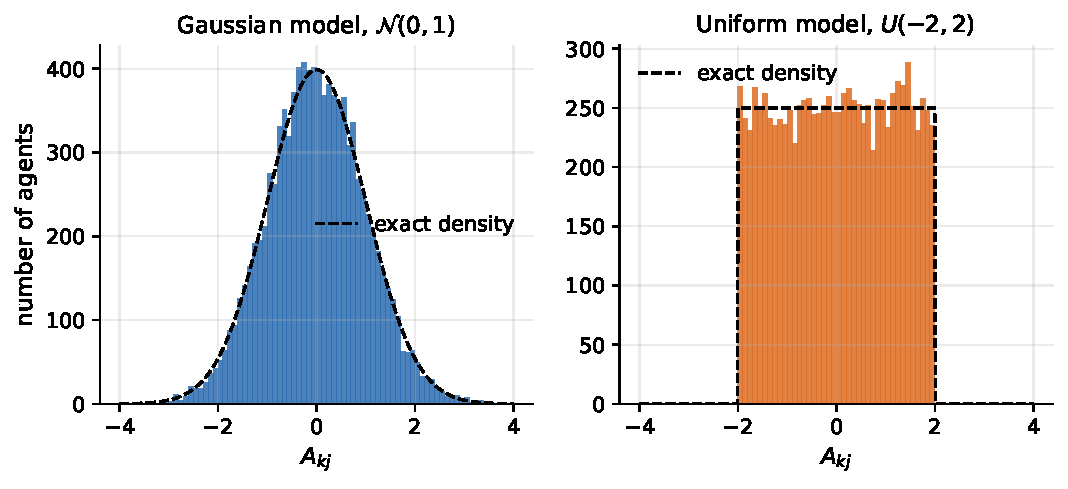
\includegraphics[width=\linewidth]{fig01_initial_histograms}
  \caption{Histogram of the values $\{A_{kj} : j \neq k\}$ for a single agent
  $k$, with bin size $0.1$, in the Gaussian and uniform models with
  $N = 10{,}000$, $\mu = 0$ and $\sigma = 1$. Dashed: the generating density.}
  \label{fig:initial}
  \Description{Two histograms of one agent's affinities for all other agents,
  one bell-shaped for the Gaussian model and one flat for the uniform model,
  each overlaid with the exact density.}
\end{figure}

The diagonal elements of the affinity matrix are the utilities of being single.
We also take these to be generated by a distribution, with density $p_0$. The
mean of the diagonal is the average utility when all agents are single; the mean
of the off-diagonal entries is the average utility when agents form random
couples. The relationship between the two therefore encodes how being single
compares with dating a random member of society. We do not believe these two
quantities are generically equal, but for concreteness we present our main
results assuming they are, and show in Section~\ref{sec:robust} that the
conclusions survive when they are not. In the analytical treatment of
Section~\ref{sec:largeN} the two distributions are kept separate throughout: we
write $p_0$ for the density generating the diagonal and $p_A$ for the density
generating the off-diagonal entries.

\subsection{Dynamics}
\label{sec:dynamics}

The dynamics happen in discrete steps $t \in \mathbb{N}$. At each step all agents
are paired at random: a random perfect matching, that is, an involution without
fixed points
%
\begin{align}
  \pi_t : \{1, 2, \dots, N\} \rightarrow \{1, 2, \dots, N\},
  \label{eq:matching}
\end{align}
%
drawn uniformly. The agent $k$ meets at step $t$ is $\pi_t(k)$. We write $u_t^k$
for the utility of agent $k$ at step $t$.

Suppose first that agent $k$ is single at $t$, so $u_t^k = A_{kk}$, and meets
agent $l = \pi_{t+1}(k)$. The two form a couple if they like each other enough:
%
\begin{align}
  u_{t+1}^k = \begin{cases}
    A_{kl}, & \text{if } A_{kl} > u_t^k \text{ and } A_{lk} > u_t^l,\\
    u_t^k, & \text{otherwise}.
  \end{cases}
  \label{eq:single}
\end{align}
%
Now suppose agent $k$ is in a couple with agent $m$ at $t$, so $u_t^k = A_{km}$
and $u_t^m = A_{mk}$. At step $t+1$ let $k$ meet $l = \pi_{t+1}(k)$ and $m$ meet
$n = \pi_{t+1}(m)$. If the affinity between newly met agents exceeds that
between the mates, a new couple forms and the old one breaks apart:
%
\begin{align}
  u_{t+1}^k = \begin{cases}
    A_{kl}, & \text{if } A_{kl} > u_t^k \text{ and } A_{lk} > u_t^l,\\
    A_{kk}, & \text{if } A_{mn} > u_t^m \text{ and } A_{nm} > u_t^n,\\
    u_t^k, & \text{otherwise}.
  \end{cases}
  \label{eq:couple}
\end{align}
%
Both comparisons are made against the utilities as of the start of the step. We
start the system with all agents single, $u_0^k = A_{kk}$. A couple here is not
a married couple; marriage is introduced in Section~\ref{sec:marriage}.

Running the simulation for $T$ steps produces an $N \times T$ array
$\{u_t^k\}$. As we are interested in large societies, $T \ll N$, we focus on the
average utility and its dispersion,
%
\begin{align}
  u_t \equiv \frac{1}{N}\sum_{k=1}^N u_t^k,
  \qquad
  \sigma_t \equiv \sqrt{\frac{1}{N}\sum_{k=1}^N (u_t^k)^2
    - \Big(\frac{1}{N}\sum_{k=1}^N u_t^k\Big)^2}.
\end{align}
%
All moments carry aggregate information; Section~\ref{sec:largeN} treats the
higher ones. The difference between $u_t^k$ and $u_t$ is visible in
Figure~\ref{fig:traj}: individual trajectories jump up when an agent finds
someone better and crash back to $A_{kk}$ when an agent is left, while the
average rises smoothly.

\begin{figure}[t]
  \centering
  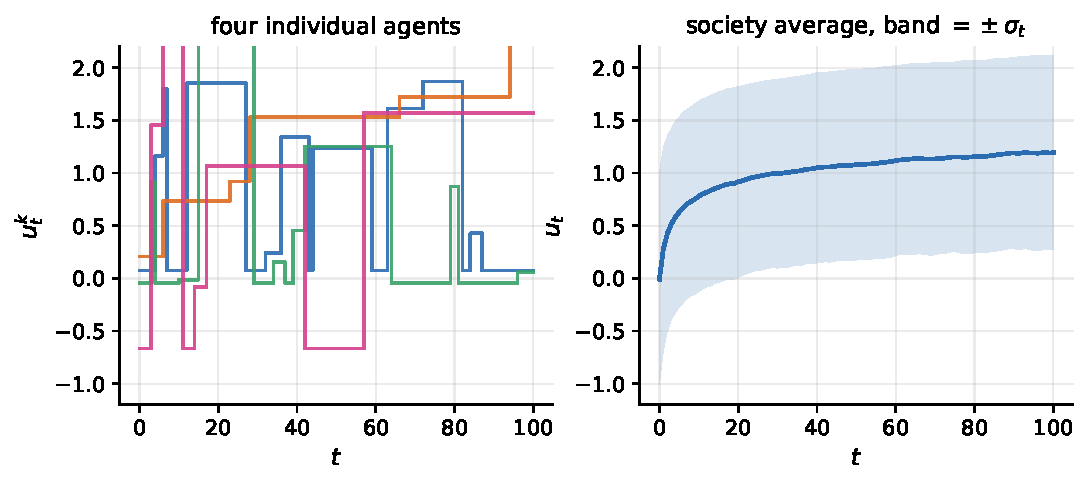
\includegraphics[width=\linewidth]{fig02_trajectories}
  \caption{Left: utility of four agents, distinguished by colour. Right: average
  utility with a band of one standard deviation. Gaussian model $\N(0,1)$,
  $N = 10{,}000$, no marriage. The uniform model $U(-2,2)$, which has the same
  variance, is visually indistinguishable.}
  \label{fig:traj}
  \Description{Left panel shows four jagged step functions rising and falling
  over time. Right panel shows a single smooth rising curve with a shaded band.}
\end{figure}

\subsection{Scale Invariance}
\label{sec:scaling}

The results we present were obtained with $\mu = 0$ and $\sigma = 1$. When all
entries of the affinity matrix come from the same distribution there is a
symmetry that carries them to generic $\mu$ and $\sigma$. Equations
\eqref{eq:single} and~\eqref{eq:couple} depend only on inequalities between
entries of $A$, so the dynamics are unchanged under the affine map
$A_{ij} \mapsto \sigma A_{ij} + \mu$. The utility of each agent transforms the
same way:
%
\begin{align}
  \text{if } (\mu = 0, \sigma = 1) \mapsto u_t^k
  \quad\text{then}\quad
  (\mu, \sigma) \mapsto \sigma u_t^k + \mu.
  \label{eq:scaling}
\end{align}
%
It therefore suffices to read $0$ as $\mu$ and to interpret the vertical axis of
every figure in units of $\sigma$.

\subsection{No Equilibrium to Converge To}

In large societies the number of new people we meet over a lifetime is much
smaller than the size of society, $T \ll N$. The asymptotic limit
$T \rightarrow \infty$ is correspondingly not the object of interest. This
resonates with Keynes's remark that ``in the long run we are all
dead''~\cite{keynes1923tract}, read as the advice that asymptotic limits and
equilibrium states are not always relevant.

More than that: in the model without marriage, the limit
$T \rightarrow \infty$ does not approach any equilibrium at all. Consider three
agents $A$, $B$ and $C$, where $A$ has highest affinity with $C$, $B$ with $C$,
and $C$ with $A$. At each step one of them is left out, and they remain in an
eternal dance---a situation not unknown in modern relationships. Because the
system never settles, even generalised notions of
stability~\cite{Multi-period, doval2021dynamically, Credibility, DAMIANO200534}
may not be the right tool for understanding how couples match in large
societies.

%%%%%%%%%%%%%%%%%%%%%%%%%%%%%%%%%%%%%%%%%%%%%%%%%%%%%%%%%%%%%%%%%%%%%%%%

\section{The Marriage Model}
\label{sec:marriage}

The marriage model extends the mate-search model as follows. We introduce the
\emph{proposal vector} $\vec{\Lambda} \in \R^N$, where $\Lambda_k$ encodes how
much agent $k$ needs to like another agent before proposing marriage. If the
affinity within a couple exceeds both members' thresholds, the couple stops
meeting new agents. We then say the couple is \emph{married}:
%
\begin{align}
  \text{the couple } (k,l) \text{ is married at } t
  \iff
  A_{kl} > \Lambda_k \ \text{ and }\ A_{lk} > \Lambda_l .
  \label{eq:married}
\end{align}
%
Let $\Mset_t \subseteq \{1, \dots, N\}$ be the set of agents married at time $t$.
The matching at time $t+1$ does not include them:
%
\begin{align}
  \pi_{t+1}^\Lambda :
  \{1, \dots, N\} \setminus \Mset_t \rightarrow
  \{1, \dots, N\} \setminus \Mset_t .
  \label{eq:marriedmatching}
\end{align}
%
Because married agents are never matched again, they can never be poached, and a
married couple never breaks. Consequently $\Mset_t$ is non-decreasing in $t$,
and $\Lambda = \infty$ recovers the mate-search model exactly.

As before, what matters for a large society is the distribution generating
$\vec{\Lambda}$, and a reasonable assumption is
$\Lambda_k \sim \N(\Lambda, \sigma_\Lambda)$. The values $\Lambda$ and
$\sigma_\Lambda$ are exogenous: they characterise the behaviour of the agents of
a given society. Different societies---or the same society at different
times---will have different values of $\Lambda$, a point we return to in
Section~\ref{sec:empirical}. To keep the investigation tractable we take the
limit $\sigma_\Lambda \rightarrow 0$ throughout, so $\Lambda_k = \Lambda$ for all
$k$.

The scaling relation~\eqref{eq:scaling} continues to hold provided $\Lambda$ is
shifted and rescaled along with the affinities. If $u_t^k$ is obtained for
$\mu = 0$, $\sigma = 1$ and threshold $\Lambda$, then
%
\begin{align}
  (\mu, \sigma, \sigma\Lambda + \mu) \mapsto \sigma u_t^k + \mu .
  \label{eq:scalingmarriage}
\end{align}
%
So the results below are generic in $\mu$ and $\sigma$, with $\Lambda$ measured
in units of $\sigma$ above the mean.

%%%%%%%%%%%%%%%%%%%%%%%%%%%%%%%%%%%%%%%%%%%%%%%%%%%%%%%%%%%%%%%%%%%%%%%%

\section{Results}
\label{sec:results}

Unless stated otherwise, all simulations use $N = 10{,}000$ agents, $T = 100$
steps, $\mu = 0$ and $\sigma = 1$. Where error bars are quoted they are standard
errors over eight independent societies. When we compare a society with marriage
against one without, both are run on the \emph{same} affinity matrix with
independent matchings, so that the difference between the two is not an artefact
of sampling~$A$.

\subsection{Marriage Can Raise Average Utility}

Figure~\ref{fig:lcomp} and Table~\ref{tab:lambda} compare the average utility
for different values of $\Lambda$. The most significant lessons of the model can
be read off from them.

\begin{figure*}[t]
  \centering
  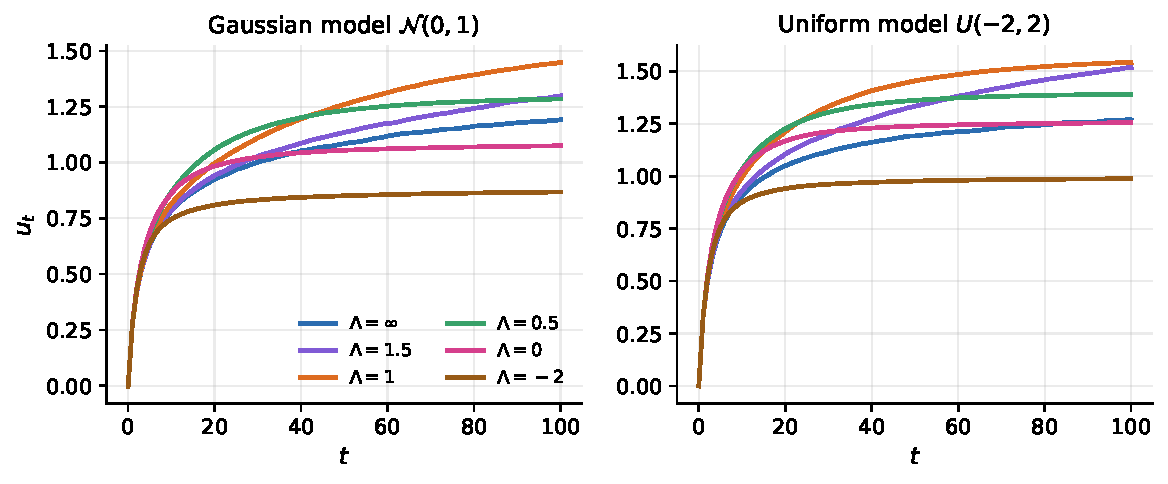
\includegraphics[width=0.86\textwidth]{fig03_lambda_comparison}
  \caption{Average utility evolution in the Gaussian and uniform models with
  $N = 10{,}000$ for different values of $\Lambda$; $\Lambda = \infty$ denotes
  the society without marriage. Mean over eight independent societies, with
  standard-error bands.}
  \label{fig:lcomp}
  \Description{Two panels, each with six rising curves. The curve for Lambda
  equal to one ends highest in both panels; the curve for Lambda equal to minus
  two ends lowest.}
\end{figure*}

\begin{table}[t]
  \caption{Average utility $u_{100}$ at the end of the run, by threshold.
  Mean $\pm$ standard error over eight societies of $N = 10{,}000$.}
  \label{tab:lambda}
  \begin{tabular}{lcc}\toprule
    \textit{Threshold} & \textit{Gaussian} $\N(0,1)$ & \textit{Uniform} $U(-2,2)$ \\ \midrule
    $\Lambda = \infty$ (no marriage) & $1.191 \pm 0.004$ & $1.269 \pm 0.003$ \\
    $\Lambda = 1.5$ & $1.298 \pm 0.003$ & $1.519 \pm 0.001$ \\
    $\Lambda = 1$   & $\mathbf{1.447 \pm 0.003}$ & $\mathbf{1.543 \pm 0.001}$ \\
    $\Lambda = 0.5$ & $1.285 \pm 0.002$ & $1.391 \pm 0.001$ \\
    $\Lambda = 0$   & $1.075 \pm 0.003$ & $1.255 \pm 0.002$ \\
    $\Lambda = -2$  & $0.868 \pm 0.002$ & $0.988 \pm 0.002$ \\ \bottomrule
  \end{tabular}
\end{table}

Two limits bracket the behaviour. If $\Lambda > A_{ij}$ for all $i, j$, marriage
never triggers and the dynamics are those of the mate-search model; for
sufficiently large $\Lambda$ at finite $N$, the two models coincide. If instead
$\Lambda < A_{ij}$ for all $i, j$, every agent marries the first agent it
likes, and the average utility drops well below the no-marriage baseline---at
$\Lambda = -2$, to $0.868$ against $1.191$. The lesson is that one should not
marry the first person one likes.

Between the two extremes something more interesting happens. For $\Lambda$ near
$\sigma$ the average utility is consistently \emph{larger} than in the society
without marriage: $1.447$ against $1.191$ in the Gaussian model, a gain of
$0.26\sigma$, and $1.543$ against $1.269$ in the uniform model. It is therefore
reasonable to conclude that one should marry if one likes one's partner more
than a sigma above average. Note also that the curves cross: the value
$\Lambda_t$ maximising average utility depends on the horizon $t$, and a society
that expects a long search should be more demanding than one that does not.

To clarify the interpretation, consider the following scenario. During our lives
we can take every opportunity to meet others, pursuing the dream of finding the
greatest love of our lives. Alternatively, having found someone who makes us
happy by more than a certain amount, we can stop searching. The model says that
on average it is better to stick with someone good enough than to keep looking.
Together with the $\Lambda = -2$ result, this justifies the advice advertised
above: do not marry the first person you like and do not search for the love of
your life, but get married if you like your partner more than a sigma above
average.

There is a second interpretation that motivated this model. Suppose you are
dating and must decide whether to engage in monogamy or non-monogamy. The most
salient difference is that in non-monogamy you and your mate remain open to
meeting others. Many features of your preferences bear on the decision: how much
you enjoy meeting new people, whether you have time for both a mate and
sporadic matches, how jealous you feel. In addition, the openness characteristic
of non-monogamous relationships increases the chance of meeting someone with
whom either you or your mate has a higher affinity. You may then wonder whether
the odds of finding someone better outweigh the risk of being left. If one reads
our couples as non-monogamy and our married couples as monogamy, the model
addresses this question and gives a negative answer. If you are in all other
respects unsure which you prefer, the benefit of marriage as a search strategy
disclosed here should tip the balance towards monogamy. This interpretation may
grow in relevance as the number of people who experience non-monogamous
relationships increases~\cite{doi:10.1080/0092623X.2016.1178675}. Throughout the
rest of the paper we stick to the first interpretation.

\subsection{Marriage Also Reduces Inequality}

It is instructive to plot the evolution of $u_t$ together with its dispersion,
as in Figure~\ref{fig:utumt}. The society with marriage at $\Lambda = \sigma$ has
both a higher mean and a \emph{lower} variance: in the Gaussian model the
standard deviation at $t = 100$ falls from $0.914$ to $0.645$, and in the uniform
model from $0.838$ to $0.371$. If agents value equality with respect to
relationships, this is a second benefit of marriage on top of the first. The
mechanism is visible in the full distributions (Figure~\ref{fig:finalhist}):
marriage imposes a floor, because every married agent is above $\Lambda$ by
construction, and it drains the mass of long-term singles sitting at their
$A_{kk}$.

\begin{figure}[t]
  \centering
  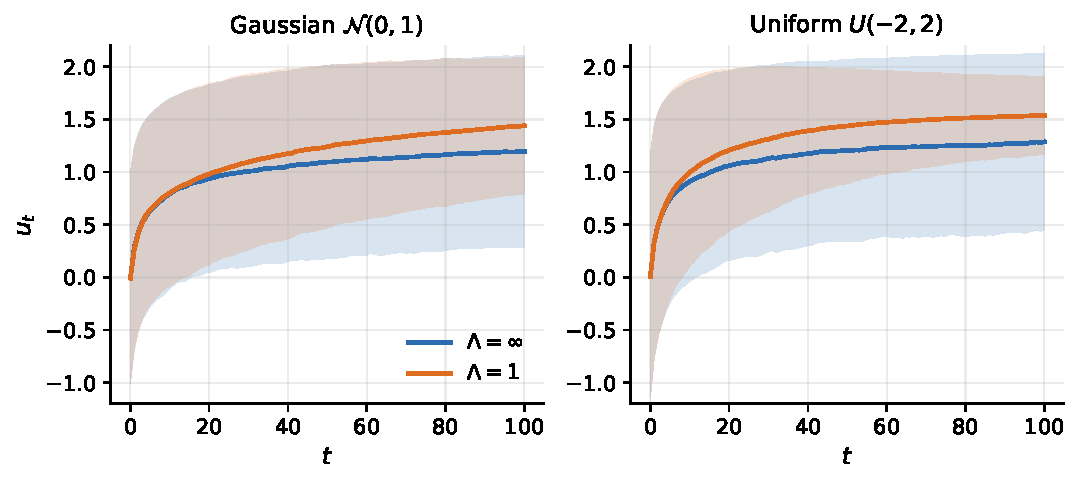
\includegraphics[width=\linewidth]{fig04_marriage_vs_none}
  \caption{Average utility with marriage at $\Lambda = 1$ (orange) and without
  marriage (blue), with bands of one standard deviation, for $N = 10{,}000$.
  Both societies share the same affinity matrix.}
  \label{fig:utumt}
  \Description{Two panels each showing an orange curve above a blue curve, with
  the orange band visibly narrower than the blue one.}
\end{figure}

\begin{figure}[t]
  \centering
  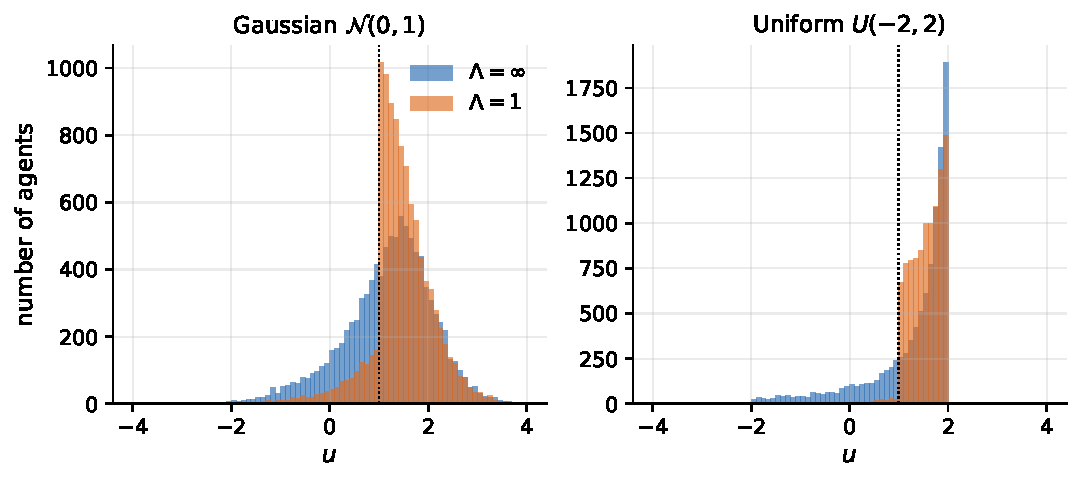
\includegraphics[width=\linewidth]{fig05_final_histograms}
  \caption{Histogram of $\{u_{100}^k\}$ with bin size $0.1$ for the society with
  marriage at $\Lambda = 1$ (orange) and without marriage (blue). Dotted line:
  the threshold $\Lambda = 1$.}
  \label{fig:finalhist}
  \Description{Two overlaid histograms per panel; the orange one is shifted to
  the right and has a sharp left edge at the threshold.}
\end{figure}

\subsection{The Price: A Shorter Search}

The benefit is bought with something. Figure~\ref{fig:partners} counts the
distinct partners each agent has over the run. Without marriage an agent cycles
through $5.15$ partners on average in the Gaussian model; with marriage at
$\Lambda = 1$, $4.04$. In the uniform model the reduction is sharper, from
$5.00$ to $2.76$. An agent who does not marry ends up on average with someone it
likes less, but it may nevertheless derive a surplus from having participated in
more relationships---a surplus this model does not represent. Conversely, it is
in general painful to break up, and that loss is not represented either, though
accounting for it would add a further benefit to the society with marriage.
Overall, the evidence suggests that marriage is beneficial in a number of
respects~\cite{doi:10.2307/2061670}.

\begin{figure}[t]
  \centering
  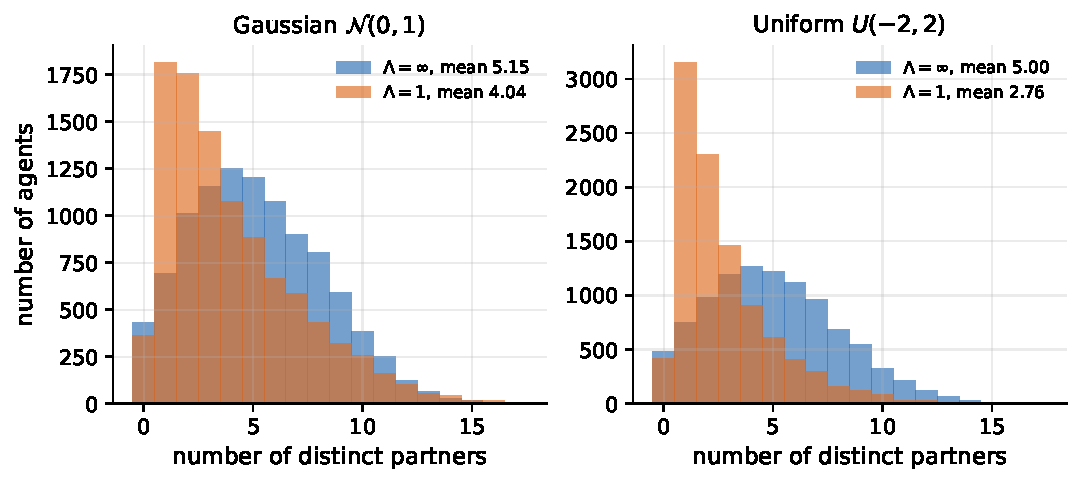
\includegraphics[width=\linewidth]{fig14_number_of_partners}
  \caption{Distinct partners per agent over $100$ steps, with and without
  marriage, $N = 10{,}000$.}
  \label{fig:partners}
  \Description{Two panels of overlaid histograms of partner counts; the orange
  with-marriage distribution is concentrated at lower counts.}
\end{figure}

\subsection{Robustness: Being Single Need Not Be the Same Draw}
\label{sec:robust}

In Section~\ref{sec:affinities} we assumed for concreteness that the diagonal and
off-diagonal elements of the affinity matrix come from the same distribution.
One might reasonably worry that the results depend on it. To address this we
simulate the model with $A_{kk} = 0$ for all $k$---being single is worth exactly
nothing---and $A_{ij} \sim \N(\mu, 1)$ for $i \neq j$, sweeping $\mu$, with the
threshold tracking the distribution at $\Lambda = \mu + \sigma$. Negative $\mu$
means most people are worse than solitude; positive $\mu$ means almost anyone
beats it. Note that $A_{kk} = 0$ is obtained formally by taking
$\sigma_s \rightarrow 0$ in the distribution generating the diagonal, and that in
this limit there is no loss of generality in setting $\sigma = 1$ off the
diagonal, since \eqref{eq:single} and~\eqref{eq:couple} remain invariant under
rescaling of $A_{ij}$ alone.

\begin{figure*}[t]
  \centering
  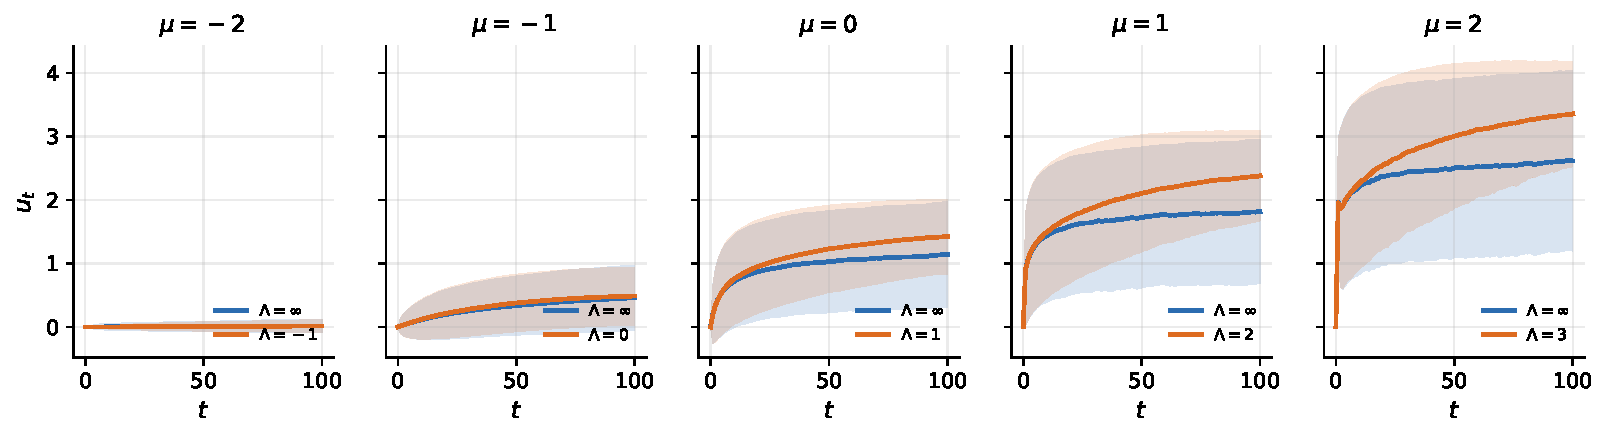
\includegraphics[width=\textwidth]{fig06_mu_robustness}
  \caption{Average utility with $A_{kk} = 0$ for all $k$ and
  $A_{ij} \sim \N(\mu,1)$ for $i \neq j$, $N = 10{,}000$. Orange: with marriage
  at $\Lambda = \mu + 1$. Blue: without marriage.}
  \label{fig:mu}
  \Description{Five panels, one per value of mu, each showing an orange curve at
  or above a blue curve, with the gap widening as mu increases.}
\end{figure*}

Figure~\ref{fig:mu} shows the outcome. Writing
$f(\mu) \equiv u_M(\mu) - u(\mu)$ for the gap between the society with marriage
and the society without, we find $f(\mu) > 0$ throughout, and $f$ non-decreasing
in $\mu$: $f(-2) = +0.001$, $f(-1) = +0.027$, $f(0) = +0.283$, $f(1) = +0.565$,
$f(2) = +0.739$. The two ends of the sweep also tell us what happens outside it.
For $\mu < -2\sigma$ an agent is unlikely to meet anyone it prefers to being
single, and the system behaves much as at $\mu = -2$. For $\mu > 2\sigma$ agents
prefer almost any partner to solitude, as at $\mu = 2$, and the dynamics are
similar up to the change of scale set by $\mu$. Since the gap is positive
throughout, the benefit of marriage is a robust feature of the model, and the
advice extracted from it holds in more general contexts.

\subsection{Who Gains, and Who Loses}
\label{sec:who}

A further objection is that the assumption of a homogeneous society is plainly
false. What is interesting is that at finite $N$ homogeneity is already broken:
each agent's column $\{A_{jk} : j \neq k\}$ is a different collection of numbers,
even though all are drawn from one distribution. One can select the $1\%$ of
agents whose column mean is largest---the most liked agents of the
society---and, conversely, the $1\%$ least liked, and follow each group
separately.

% >>> CHANGED FROM ORIGINAL. The original paper claimed, from a single run with
% ~50 agents per group, that marriage benefits the less-liked more. At N = 10^4
% the column means are spread by only 1/sqrt(N) ~ 0.01 sigma, and over six
% replicates the two premia are statistically indistinguishable
% (+0.219 +/- 0.045 against +0.254 +/- 0.043). The claim is recovered, and
% strengthened, once genuine desirability heterogeneity is added. See
% ../../FINDINGS.md section 3 and scripts/fig07_liked_disliked.py.
This, however, is asking more of finite-size effects than they can deliver. With
$N = 10{,}000$ i.i.d.\ entries, column means are spread by only
$1/\sqrt{N} \approx 0.01\sigma$, so the ``$1\%$ most liked'' are more liked by
about $0.03\sigma$. Over six independent societies the marriage premium is
$+0.219 \pm 0.045$ for the least liked and $+0.254 \pm 0.043$ for the most
liked: indistinguishable. In the homogeneous model there is no such effect to
find.

To ask the question properly the model has to be given genuine \emph{vertical}
heterogeneity. We therefore add a per-agent desirability $q_k$ to every entry of
agent $k$'s column,
%
\begin{align}
  A_{ij} = \varepsilon_{ij} + q_j,
  \qquad
  \varepsilon_{ij} \sim \N(0, \sigma_\varepsilon),
  \qquad
  q_j \sim \N(0, \sigma_q),
  \label{eq:quality}
\end{align}
%
holding the total variance $\sigma_\varepsilon^2 + \sigma_q^2 = 1$ fixed so that
runs at different $\sigma_q$ remain comparable. Now some agents really are more
widely liked than others, and $\sigma_q$ tunes how much.

\begin{figure*}[t]
  \centering
  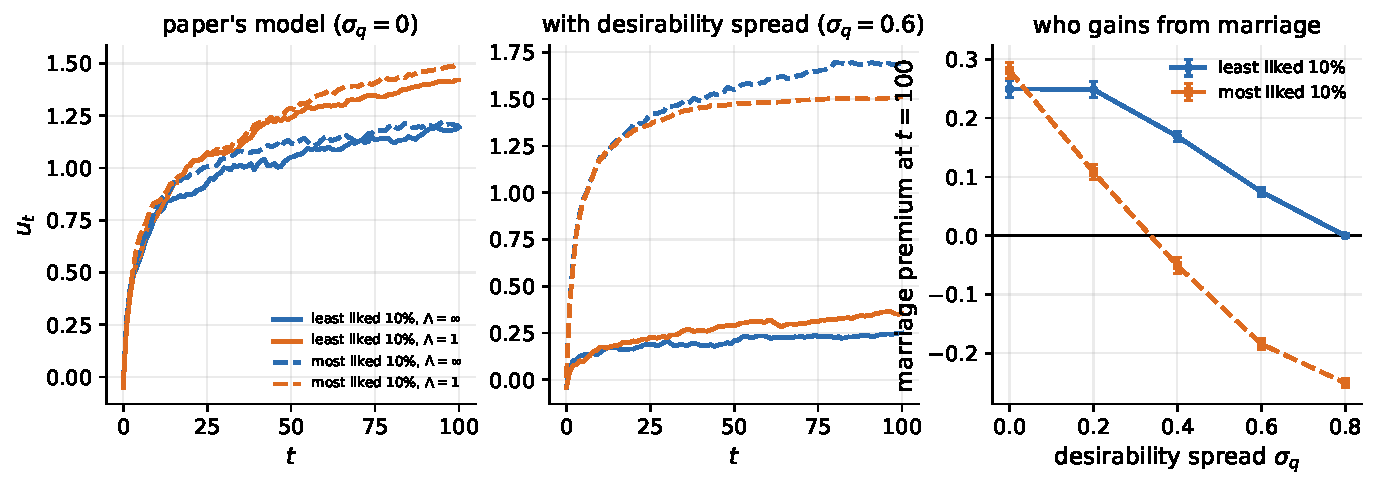
\includegraphics[width=\textwidth]{fig07_liked_disliked}
  \caption{Marriage premium at $t = 100$ for the most and least liked $10\%$ of
  agents. Left: the homogeneous model, $\sigma_q = 0$, where the two groups are
  indistinguishable. Centre: with desirability spread $\sigma_q = 0.6$. Right:
  the premium as a function of $\sigma_q$, mean $\pm$ standard error over six
  societies. Past $\sigma_q \approx 0.4$ the premium for the most desirable
  agents is negative.}
  \label{fig:who}
  \Description{Three panels. The rightmost shows two curves: the least-liked
  premium declining from positive towards zero, and the most-liked premium
  crossing from positive to negative as sigma_q increases.}
\end{figure*}

Figure~\ref{fig:who} and Table~\ref{tab:who} show the result. The paper's
original intuition is vindicated: marriage does help the less desirable more.
But the effect is stronger than ``more''. Past $\sigma_q \approx 0.4$ the
premium for the most desirable agents turns \emph{negative}: they are made
strictly worse off by living in a society that marries. The reading is
straightforward once stated. Marriage in this model is insurance against being
left. Agents whom everyone likes are rarely at risk of being left, so the
insurance is worth little to them, while the option value they give up---the
chance of meeting someone even better, which for them is a realistic
prospect---is worth a great deal.

\begin{table}[t]
  \caption{Marriage premium $u_M - u$ at $t = 100$ by desirability spread
  $\sigma_q$, for the most and least liked $10\%$ of agents. Total variance of
  $A_{ij}$ held at $1$. Mean $\pm$ standard error over six societies.}
  \label{tab:who}
  \begin{tabular}{lcc}\toprule
    $\sigma_q$ & \textit{Least liked} $10\%$ & \textit{Most liked} $10\%$ \\ \midrule
    $0.0$ & $+0.250 \pm 0.015$ & $+0.281 \pm 0.014$ \\
    $0.2$ & $+0.249 \pm 0.014$ & $+0.108 \pm 0.013$ \\
    $0.4$ & $+0.169 \pm 0.009$ & $-0.051 \pm 0.013$ \\
    $0.6$ & $+0.075 \pm 0.008$ & $-0.184 \pm 0.009$ \\
    $0.8$ & $-0.000 \pm 0.003$ & $-0.251 \pm 0.008$ \\ \bottomrule
  \end{tabular}
\end{table}

This matters for how the advice of Section~\ref{sec:results} should be read. The
benefit of marriage is not society-wide once agents differ in desirability;
there is a distributional conflict, and the agents who do best out of the
search process are precisely the ones with an incentive to defect from the
convention. A society-level threshold $\Lambda$ is therefore not obviously
self-enforcing, which is a question this model is well placed to ask and which we
leave for future work.

\subsection{Men, Women, and Other Partitions}

A possible point of concern is that we did not distinguish men from women, as in
the original marriage problem~\cite{10.2307/2312726}; one might think we are
dealing with the stable roommates problem instead. The distinction turns out not
to matter here. We can partition the society in two and match only across the
partition. The evolution of average utility for such a system is
indistinguishable from Figure~\ref{fig:utumt}: averaging over four societies, the
two-sided variant differs from the one-sided one by less than $0.03$, well inside
the run-to-run spread.

One can even partition the society into groups of different sizes, and the
results are still very similar. In that case the matching
in~\eqref{eq:matching} is a random injection from the smaller partition into the
larger, and a random subset of the larger group sits out each step. Several
further variations are possible: one could select a subset of one partition and
allow it to match within itself as well, which admits a reading as bisexual
agents. This flexibility is in line with the diversity of modern relationships,
and contrasts with results for the matching problem---many of them, including
Gale--Shapley, depend on the two sides having the same number of
elements~\cite{roth1992two}.

%%%%%%%%%%%%%%%%%%%%%%%%%%%%%%%%%%%%%%%%%%%%%%%%%%%%%%%%%%%%%%%%%%%%%%%%

\section{Comparison with Centralised Benchmarks}
\label{sec:benchmarks}

It is instructive to compare the average utility attained by the dynamics with
what a central planner could achieve on the same affinity matrix. We use three
reference points, all computed by splitting the society into two equal halves
and matching across them, which is the setting Gale--Shapley is defined for:
random pairing, which is the floor; the proposer-optimal stable
matching~\cite{10.2307/2312726}, with average utility $u_{G\text{-}S}$; and the
matching $\pi^*$ maximising total surplus,
%
\begin{align}
  u(\pi) = \frac{1}{2}\sum_{i=1}^N \big(A_{i\pi(i)} + A_{\pi(i)i}\big),
  \label{eq:becker}
\end{align}
%
which is Becker's paradigm of transferable
utility~\cite{10.2307/1831130, 10.2307/1829987}. Such a $\pi^*$ need not be
stable, but by construction it maximises average utility.

% >>> CHANGED FROM ORIGINAL (1). The original paper called the utilitarian
% optimum computationally impossible, counting N! matchings. It is a linear
% assignment problem, solvable exactly by the Hungarian algorithm in O(N^3).
% >>> CHANGED FROM ORIGINAL (2). The original reported u_GS ~ 4 for the Gaussian
% model at N ~ 1000. We obtain 1.79. See ../../FINDINGS.md section 4.
A remark on computing $\pi^*$. Naively there are $N!$ matchings to consider,
which for $N \approx 1000$ is a number with $2568$ digits. But maximising
\eqref{eq:becker} is a linear assignment problem on the symmetrised surplus
$A_{ij} + A_{ji}$, so the Hungarian algorithm solves it exactly in $O(N^3)$
time. We report it up to $N = 2000$.

\begin{figure}[t]
  \centering
  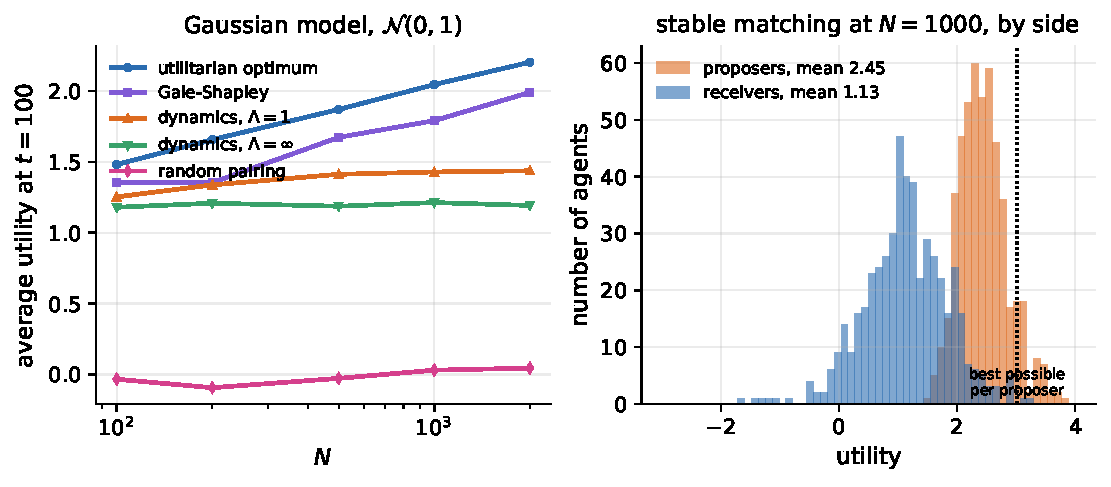
\includegraphics[width=\linewidth]{fig13_benchmarks}
  \caption{Left: average utility at $t = 100$ for the dynamics, against random
  pairing, the stable matching and the utilitarian optimum, as a function of
  $N$. Right: the two sides of the stable matching at $N = 1000$ do very
  different things.}
  \label{fig:bench}
  \Description{Left panel: five curves against N on a log axis, with the
  utilitarian optimum highest and random pairing flat near zero. Right panel:
  two overlaid histograms with clearly different means.}
\end{figure}

Figure~\ref{fig:bench} collects the comparison. At $N = 1000$ in the Gaussian
model the dynamics reach $1.213$ without marriage and $1.429$ with marriage at
$\Lambda = 1$; the stable matching reaches $u_{G\text{-}S} = 1.791$ and the
utilitarian optimum $2.045$. Random pairing gives $0.030$, i.e.\ $\mu$, as it
must. The planner's advantage grows with $N$, since both centralised benchmarks
have more to work with as the society grows while the dynamics are limited by
$T$.

Two observations follow. First, a stable matching does much better than the
decentralised process, which is one indication that the concept of stability is
not what organises matching in large societies. Second, and more usefully, the
fact that $u_{G\text{-}S}$ exceeds $u_t$ at $t \approx 100$ implies that the
market for relationships in large societies is substantially sub-optimal. If
affinities could be inferred from manifest, correlated properties---age,
personality, political leaning, level of education---then a central mechanism
could propose a stable matching and society's average utility with respect to
relationships would be considerably higher.

The right panel of Figure~\ref{fig:bench} adds a caveat that bears on how large
that gap really is. A proposer-optimal stable matching is far from symmetric
between the two sides: at $N = 1000$ the proposing side averages $2.454$ while
the receiving side averages $1.128$, and $u_{G\text{-}S}$ is the average of the
two. For reference, the mean best-possible partner for a proposer is $3.015$, so
no matching of any kind can place the two-sided average near it. Any claim about
the size of the planner's advantage should therefore say which side of the
market it is talking about.

%%%%%%%%%%%%%%%%%%%%%%%%%%%%%%%%%%%%%%%%%%%%%%%%%%%%%%%%%%%%%%%%%%%%%%%%

\section{The Large-Population Limit}
\label{sec:largeN}

So far we have focused on the average utility and its variance, which are
aggregates of the set $\{u_t^k\}$. That set carries a great deal more
information, as the histograms of Figure~\ref{fig:finalhist} show. A convenient
way to collect it is to introduce a random variable $U_t$ taking the values
$\{u_t^k\}$ each with probability $1/N$. The average utility is then $\E[U_t]$
and the variance $\E[U_t^2] - \E[U_t]^2$, where
%
\begin{align}
  \E[U_t^n] \equiv \frac{1}{N}\sum_{k=1}^N (u_t^k)^n .
\end{align}
%
This makes precise what is lost by looking only at the mean and variance: the
higher moments of $U_t$.

At $t = 0$ we have $u_0^k = A_{kk} \sim U_0$, with known density $p_0$, so in the
limit $N \rightarrow \infty$,
%
\begin{align}
  \E[U_0^n] = \lim_{N \rightarrow \infty} \frac{1}{N}\sum_{k=1}^N A_{kk}^n
  = \int_{-\infty}^{\infty} u^n p_0(u)\, du,
\end{align}
%
and we have complete information about the system. The density $p_t(u)$ that
generates the values $\{u_t^k\}$ is thus more fundamental than the values
themselves. Given $p_t$ one obtains $\E[U_t^n]$ by integration; given all the
moments one recovers $p_t$ by computing the characteristic function
%
\begin{align}
  \E[e^{\imath k U_t}] = \int_{-\infty}^\infty e^{\imath k u} p_t(u)\, du
  = \sum_{n=0}^\infty \E[U_t^n]\frac{(\imath k)^n}{n!}
  \label{eq:charfn}
\end{align}
%
and inverting the Fourier transform. Finding $p_{t+1}$ from $p_t$ is therefore
equivalent to finding $\E[U_{t+1}^n]$ from $\E[U_t^n]$, and that is the task of
this section.

Before starting, one caveat. Although more tractable and in a sense more
fundamental, the continuum version lacks a feature that the finite
implementation shares with reality. At $N \rightarrow \infty$ the society is
genuinely homogeneous, whereas at finite $N$ some agents are more liked than
others---and, as Section~\ref{sec:who} showed, in real societies they are more
liked by considerably more than sampling noise would give. The analysis of
Section~\ref{sec:who} has no counterpart in the continuum theory as set up here.

\subsection{Decomposition into Couples and Singles}

Agents are either coupled or single at each step, and the two behave differently,
so $p_t$ decomposes as
%
\begin{align}
  p_t(u) = b_t\, p_{ct}(u) + r_t\, p_{st}(u),
  \label{eq:decomposition}
\end{align}
%
with $p_{ct}$ and $p_{st}$ the utility densities of coupled and single agents and
$b_t, r_t$ their population shares, $b_t + r_t = 1$. Introducing random variables
$C_t$ and $S_t$ for couples and singles, \eqref{eq:decomposition} is equivalent
to
%
\begin{align}
  \E[U_t^n] = b_t\, \E[C_t^n] + r_t\, \E[S_t^n] .
  \label{eq:moments}
\end{align}
%
At $t = 0$ all agents are single, so $b_0 = 0$, $r_0 = 1$ and $S_0 \sim U_0$.

Write $F_A$ for the cumulative distribution function of $p_A$ and
$\bar{G}_A = 1 - F_A$ for its survival function, so that $\bar{G}_A(x)$ is the
probability that a random agent's affinity for you exceeds $x$. Three scalars
recur throughout:
%
\begin{align}
  \alpha_t &\equiv \E_{L \sim U_t}\big[\bar{G}_A(L)\big], \label{eq:alpha}\\
  \gamma_t &\equiv \E_{M \sim C_t}\big[\bar{G}_A(M)\big], \label{eq:gamma}\\
  \beta_t &\equiv 1 - \alpha_t \gamma_t . \label{eq:beta}
\end{align}
%
In words: $\alpha_t$ is the probability that a random agent accepts you,
$\gamma_t$ the same restricted to agents currently in a couple, and $\beta_t$
the probability that your own partner is \emph{not} poached this step.

\subsection{Warm-Up: The First Step}
\label{sec:firststep}

At $t = 1$ all agents start single, so only $\alpha_0$ is needed. Two single
agents $K$ and $L$ form a couple if each likes the other more than being single,
an event of probability
%
\begin{align}
  c_0(K, L) \equiv \bar{G}_A(K)\, \bar{G}_A(L),
  \label{eq:c0}
\end{align}
%
and the fraction of agents in a couple at $t = 1$ is
$b_1 = \E[c_0(K,L)]$ with $K, L \sim U_0$. For the homogeneous models, in which
$p_0 = p_A$, this gives
%
\begin{align}
  b_1 = \tfrac{1}{4}, \qquad r_1 = \tfrac{3}{4} .
  \label{eq:b1r1}
\end{align}
%
In a typical simulation of the uniform model with $N = 10{,}000$ we obtain
$b_1^{\mathrm{exp}} = 0.2450$, and at $N = 200{,}000$, $b_1^{\mathrm{exp}}
= 0.2502$.

Conditioning on the couple forming, the new utility of $K$ is distributed as
$p_A$ restricted to lie above $K$'s previous utility. Taking the expectation
over $K \sim S_t$ and $L \sim U_t$ gives the densities directly:
%
\begin{align}
  b_1 p_{c1}(u) &= \alpha_0\, p_A(u)\, F_{S_0}(u), \label{eq:pc1raw}\\
  r_1 p_{s1}(u) &= p_{s0}(u)\,\big[\alpha_0 F_A(u) + 1 - \alpha_0\big].
  \label{eq:ps1raw}
\end{align}
%
The second line says a single stays single either because the agent it met
rejected it, or because it rejected the agent it met. For the uniform model,
where $p_0 = p_A = 1/(4\sigma)$ on $[-2\sigma, 2\sigma]$, this evaluates to
%
\begin{align}
  p_{c1}(u) = \frac{2\sigma + u}{2\sigma}\, p_0(u),
  \qquad
  p_{s1}(u) = \frac{6\sigma + u}{6\sigma}\, p_0(u),
  \label{eq:pc1ps1}
\end{align}
%
whose weighted sum is
%
\begin{align}
  p_1(u) = b_1 p_{c1}(u) + r_1 p_{s1}(u) = \frac{4\sigma + u}{4\sigma}\, p_0(u).
  \label{eq:p1}
\end{align}
%
Figure~\ref{fig:firststep} compares these against the simulated histograms.

\begin{figure}[t]
  \centering
  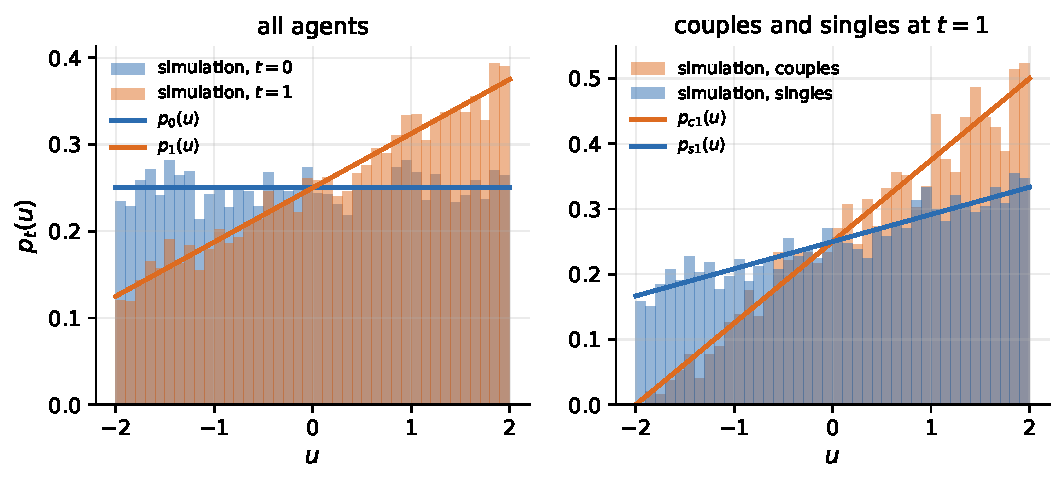
\includegraphics[width=\linewidth]{fig09_first_step_distributions}
  \caption{Exact densities after one step in the uniform model, against
  simulated histograms at $N = 10{,}000$. Left: all agents at $t = 0$ and
  $t = 1$. Right: couples and singles separately at $t = 1$.}
  \label{fig:firststep}
  \Description{Two panels, each with histograms overlaid by straight-line
  densities that follow them closely.}
\end{figure}

The mean after one step follows in closed form for both models:
%
\begin{align}
  \E[U_1] = \begin{dcases}
    \dfrac{\sigma}{2\sqrt{\pi}}, & \text{Gaussian},\\[1ex]
    \dfrac{\sigma}{3}, & \text{uniform},
  \end{dcases}
  \label{eq:EU1}
\end{align}
%
both consistent with the scaling relation~\eqref{eq:scaling}. The simulation at
$N = 10{,}000$ gives $0.2785$ against $1/(2\sqrt{\pi}) = 0.2821$.

\subsection{Evolution Equations}
\label{sec:evolution}

For $t \geq 1$ some agents are coupled, and a coupled agent has two ways to end
the step still coupled: it forms a new couple, or it keeps the one it has,
which requires that its partner was not poached. Collecting the cases and
writing the result directly in density form,
%
\begin{align}
  b_{t+1}\, p_{c,t+1}(u)
  &= \alpha_t\, p_A(u)\,\big[b_t F_{C_t}(u) + r_t F_{S_t}(u)\big] \notag\\
  &\quad + \beta_t\, b_t\, p_{ct}(u)\,\big[\alpha_t F_A(u) + 1 - \alpha_t\big],
  \label{eq:evolc}\\[1ex]
  r_{t+1}\, p_{s,t+1}(u)
  &= \alpha_t \gamma_t \beta_t\, b_t\, p_0(u) \notag\\
  &\quad + r_t\, p_{st}(u)\,\big[\alpha_t F_A(u) + 1 - \alpha_t\big].
  \label{eq:evols}
\end{align}
%
The first line of \eqref{eq:evolc} covers new couples, formed by an agent---
coupled or single---out-bidding whatever it had, with the new utility drawn from
$p_A$ above the old one. The second line covers survival. The first line of
\eqref{eq:evols} is the inflow of agents whose partner left them, who revert to
their single utility and so re-enter distributed as $p_0$; the second is singles
who stayed single. Integrating recovers $b_{t+1}$ and $r_{t+1}$, and since
$c_0 + s_0 = 1$ identically, $b_{t+1} + r_{t+1} = b_t + r_t$, so probability is
preserved by induction.

For the uniform model every density stays a polynomial, and the recursion can be
carried out exactly in rational arithmetic. At $t = 2$,
%
\begin{align}
  b_2 = \frac{1861}{5184}, \qquad r_2 = \frac{3323}{5184},
  \label{eq:b2}
\end{align}
%
with
%
\begin{align}
  p_{c2}(u) &= \frac{3(2\sigma + u)(2258\sigma + 335u)}{7444\,(2\sigma)^3},
  \label{eq:pc2}\\
  p_{s2}(u) &= \frac{3233(2\sigma)^2 + 3672\sigma u + 270u^2}{6646\,(2\sigma)^3}.
  \label{eq:ps2}
\end{align}
%
Further steps can be computed, but the coefficients grow explosively: the exact
$b_4$ is a ratio of $35$-digit integers. Figure~\ref{fig:pt} plots $p_t$ for
$t = 0, \dots, 4$ and compares $p_2$ with the simulated histogram.

\begin{figure*}[t]
  \centering
  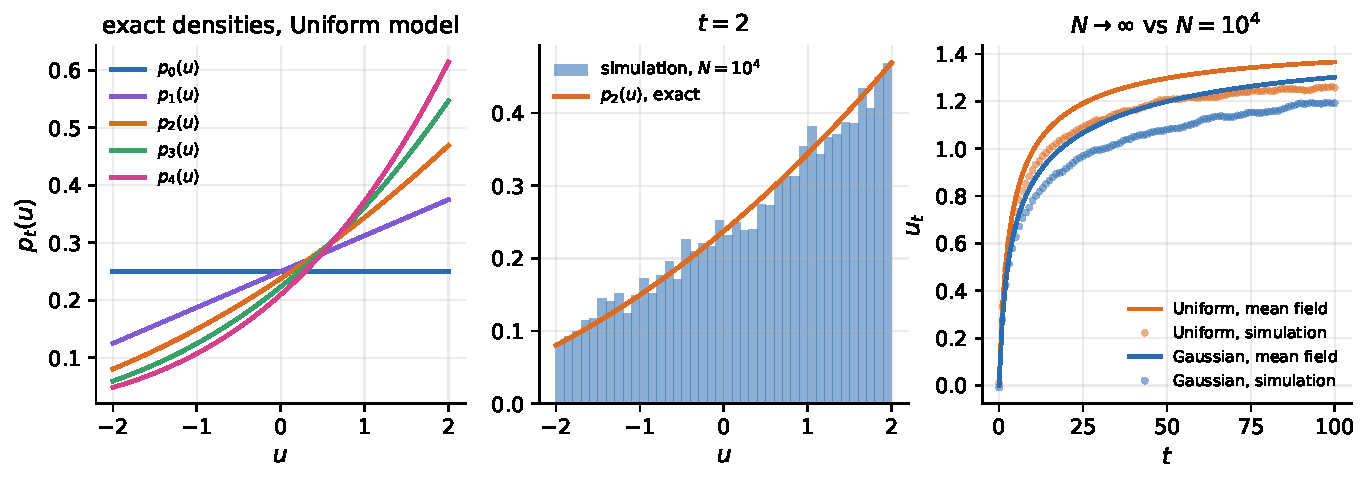
\includegraphics[width=\textwidth]{fig10_pt_evolution}
  \caption{Left: exact densities $p_t(u)$ for $t = 0, \dots, 4$ in the uniform
  model. Centre: $p_2(u)$ against the simulated histogram at $N = 10{,}000$.
  Right: the mean-field mean utility against simulation for both models.}
  \label{fig:pt}
  \Description{Three panels: a family of increasingly tilted densities, a
  histogram matched by a quadratic curve, and two pairs of curves that agree
  early and separate later.}
\end{figure*}

\subsection{Where the Mean-Field Description Is Valid}
\label{sec:mfvalid}

% >>> CHANGED FROM ORIGINAL. The original paper left the validity of these
% equations as an open question ("we do not know how to rigorously prove that
% this system of equations is indeed the N -> infinity limit ... it may be the
% case that there are higher-order effects that we are not considering").
% This subsection settles it negatively. See ../../FINDINGS.md section 2 and
% scripts/fig11_meanfield_validation.py.
Equations \eqref{eq:evolc} and~\eqref{eq:evols} were derived by an intuitive
argument, and it is natural to ask whether they really describe the
$N \rightarrow \infty$ limit. Because the affinity matrix need not be stored
explicitly---entries can be generated on demand from a counter-based hash of
$(i,j)$, which keeps them fixed and reproducible at $O(N)$ memory---we can
simulate societies of $N = 10^6$, that is, an affinity matrix with $10^{12}$
entries. At that size sampling noise is negligible and any residual disagreement
belongs to the theory.

\begin{figure*}[t]
  \centering
  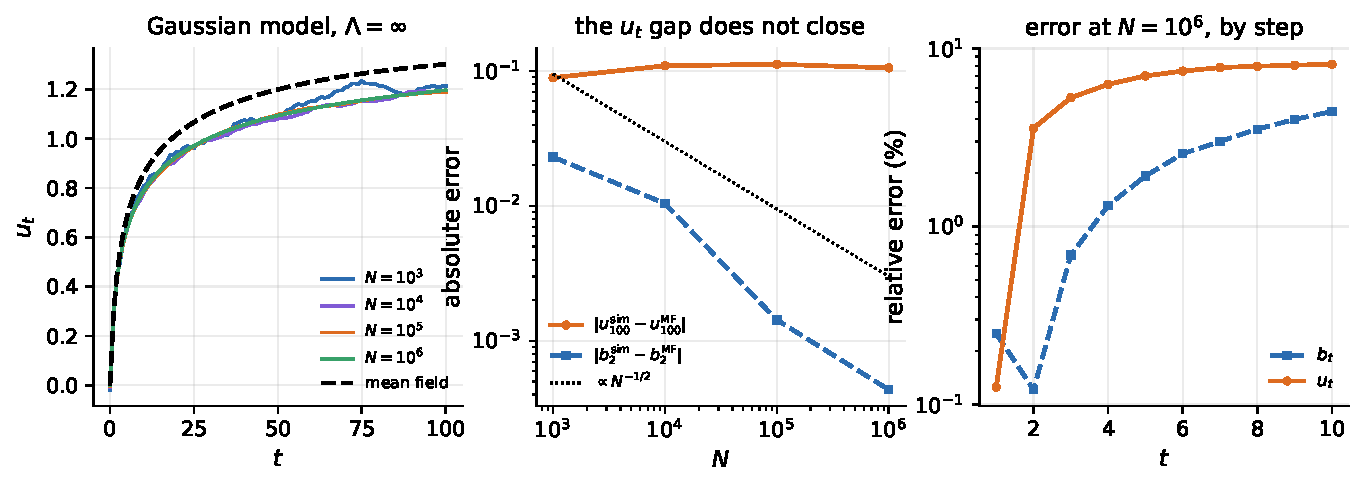
\includegraphics[width=\textwidth]{fig11_meanfield_validation}
  \caption{Left: average utility from simulation at increasing $N$, against the
  mean-field prediction. Centre: the error in $u_{100}$ is flat in $N$ while the
  error in $b_2$ falls as $N^{-1/2}$. Right: relative error at $N = 10^6$ by
  step; the deficit appears at $t = 2$.}
  \label{fig:mfvalid}
  \Description{Three panels showing that simulated curves at several N collapse
  onto one another but sit below the dashed mean-field curve.}
\end{figure*}

The answer, shown in Figure~\ref{fig:mfvalid}, is mixed. The occupancy is
predicted correctly: $b_2$ converges to $1861/5184$ as $N^{-1/2}$, and at
$N = 10^6$ agrees to $0.12\%$. The first step is predicted correctly in every
respect, with $u_1$ accurate to $0.13\%$. But from $t = 2$ onwards the mean
utility is systematically over-predicted---by $3.6\%$ at $t = 2$, $5.3\%$ at
$t = 3$, and around $8\%$ by $t = 100$---and the discrepancy does \emph{not}
shrink as $N$ grows from $10^3$ to $10^6$. It is a bias, not a finite-size
effect.

The source is an independence assumption. In deriving \eqref{eq:evolc} the two
members of a couple are treated as independent draws from $C_t$. They are not:
a couple exists precisely because each member cleared the other's threshold, so
their utilities are correlated from the moment it forms, and the correlation
compounds as the couple survives successive steps. Population shares are
insensitive to this over a single step, which is why $b_2$ comes out right; the
shape of the density is not. A correct treatment would track the joint density
of a couple, $p_{ct}(u, v)$, rather than its marginal---at the cost of turning a
one-dimensional recursion into a two-dimensional one. We leave this to future
work, and read Figure~\ref{fig:mfvalid} as delimiting where the present
equations may be trusted: exactly at $t = 1$, for occupancy at $t = 2$, and as
an upper bound on $u_t$ thereafter.

\subsection{The Distribution of Married Couples}
\label{sec:pinf}

In the model with marriage, married couples decouple from the system: they are
never selected by the matching~\eqref{eq:marriedmatching}, so they never break,
and once an agent is married its utility is frozen. This alone determines the
utility distribution of married couples, and shows it to be the same at every
step. As the system evolves an ever larger fraction of agents is married, until
in the limit all are, so the asymptotic distribution
%
\begin{align}
  p_\infty(u) \equiv \lim_{t \rightarrow \infty} p_t(u)
\end{align}
%
is also the distribution of married couples at each step.

Consider first an agent whose current utility is below $\Lambda$. Eventually it
meets an agent it likes by more than $\Lambda$, mutually, and marries. Its final
utility is therefore $p_0$ conditioned on exceeding $\Lambda$, and the weight of
this group is $F_0(\Lambda)$. An agent already at $x > \Lambda$---necessarily
unmarried, so its current partner is below \emph{its} threshold---must instead
clear $x$ to move, giving $p_0$ conditioned on exceeding $x$. Integrating over
$x$ yields
%
\begin{align}
  p_\infty(u) = \Theta(u - \Lambda)\, p_0(u)
  \left[
    \int_\Lambda^u \frac{p_0(x)}{\bar{G}_0(x)}\,dx
    + \frac{F_0(\Lambda)}{\bar{G}_0(\Lambda)}
  \right].
  \label{eq:pinf}
\end{align}
%
% >>> CHANGED FROM ORIGINAL. The original evaluated this integral only for the
% uniform model. Writing p_0 = -dGbar/dx makes it elementary for any p_0, which
% generalises the closed form to the Gaussian model.
The remaining integral is elementary for \emph{any} $p_0$, since
$p_0 = -\,\mathrm{d}\bar{G}_0/\mathrm{d}x$:
%
\begin{align}
  \int_\Lambda^u \frac{p_0(x)}{\bar{G}_0(x)}\,dx
  = \ln\frac{\bar{G}_0(\Lambda)}{\bar{G}_0(u)} .
  \label{eq:logidentity}
\end{align}
%
So \eqref{eq:pinf} is closed-form in general. It is normalised, since
%
\begin{align}
  \int_{-\infty}^{\infty} p_\infty(u)\,du
  = \bar{G}_0(\Lambda) + F_0(\Lambda) = 1 .
\end{align}
%
For the uniform model, where $\bar{G}_0(x) = (2\sigma - x)/(4\sigma)$, this
reduces to
%
\begin{align}
  p_\infty(u) = \Theta(u - \Lambda)\, p_0(u)
  \left[
    \ln\!\left(\frac{2\sigma - \Lambda}{2\sigma - u}\right)
    + \frac{\Lambda + 2\sigma}{2\sigma - \Lambda}
  \right].
  \label{eq:pinfuniform}
\end{align}

\begin{figure*}[t]
  \centering
  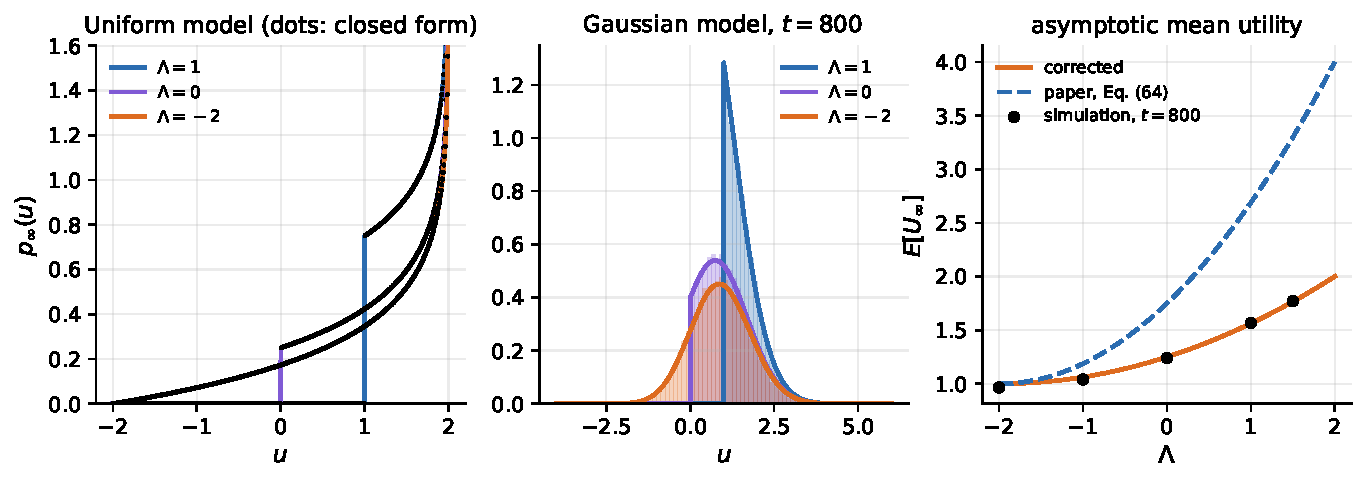
\includegraphics[width=\textwidth]{fig12_p_infinity}
  \caption{Left: $p_\infty(u)$ for the uniform model at $\sigma = 1$ and
  $\Lambda = 1, 0, -2$; dots mark the closed form~\eqref{eq:pinfuniform}.
  Centre: the same for the Gaussian model, against simulated histograms of
  married agents at $t = 800$. Right: the asymptotic mean against $\Lambda$.}
  \label{fig:pinf}
  \Description{Three panels. The left shows densities with a logarithmic
  divergence at the right edge of the support; the right shows two curves, one
  matching simulation points and one well above them.}
\end{figure*}

% >>> CHANGED FROM ORIGINAL. The original paper reported
% E[U_inf] = 3 L^2/(16 s) + 3 L/4 + 7 s/4, with maximum 4 sigma at L = 2 sigma.
% Integrating u p_inf(u) over the paper's own ansatz gives the expression below.
% The two agree only at L = -2 sigma, the single value the original checked.
% Simulation at t = 800 confirms the corrected formula at five values of Lambda.
% See ../../FINDINGS.md section 1 and scripts/fig12_p_infinity.py.
The first term of \eqref{eq:pinfuniform} diverges logarithmically as
$u \rightarrow 2\sigma$, but integrably, so moments are well defined. For the
uniform model the mean is
%
\begin{align}
  \E[U_\infty]
  = \frac{\Lambda^2}{16\sigma} + \frac{\Lambda}{4} + \frac{5\sigma}{4},
  \label{eq:EUinf}
\end{align}
%
which gives $\sigma$ at $\Lambda = -2\sigma$, as it must---every agent marries
the first partner it likes, and the average lands one sigma above the mean. It
is increasing in $\Lambda$ on the support, attaining $2\sigma$ at
$\Lambda = 2\sigma$. Expression~\eqref{eq:EUinf} is consistent with the scaling
relation~\eqref{eq:scalingmarriage}, since
$\sigma\,\E[U_\infty]\big|_{\sigma = 1, \Lambda} = \E[U_\infty]\big|_{\sigma,
\sigma\Lambda}$.

Table~\ref{tab:pinf} checks \eqref{eq:EUinf} against long simulations. The right
panel of Figure~\ref{fig:pinf} shows the same comparison graphically.

\begin{table}[t]
  \caption{Asymptotic mean utility of married agents in the uniform model:
  Equation~\eqref{eq:EUinf} against simulation at $N = 20{,}000$, $t = 800$, by
  which point $97\%$ of agents are married.}
  \label{tab:pinf}
  \begin{tabular}{lcc}\toprule
    $\Lambda$ & \textit{Eq.~\eqref{eq:EUinf}} & \textit{Simulation} \\ \midrule
    $-2$   & $1.0000$ & $0.966$ \\
    $-1$   & $1.0625$ & $1.040$ \\
    $0$    & $1.2500$ & $1.240$ \\
    $1$    & $1.5625$ & $1.567$ \\
    $1.5$  & $1.7656$ & $1.770$ \\ \bottomrule
  \end{tabular}
\end{table}

Two remarks. First, $\E[U_\infty]$ is increasing in $\Lambda$, which might
naively suggest that a society should set its threshold as high as possible.
That is not true at any finite horizon, as Figure~\ref{fig:lcomp} shows: at
$t \approx 100$ the optimum is near $\Lambda = \sigma$, and $\Lambda = 1.5$
already does worse. The asymptotic regime is reached only by waiting
arbitrarily long, which is a clean illustration of the Keynes remark quoted
earlier. Second, the size of the prize is modest. At $\Lambda = \sigma$ the
asymptotic value is $1.5625\sigma$, and the dynamics reach $1.543\sigma$ in the
uniform model by $t = 100$ already. The long run is worth much less here than
one might expect.

%%%%%%%%%%%%%%%%%%%%%%%%%%%%%%%%%%%%%%%%%%%%%%%%%%%%%%%%%%%%%%%%%%%%%%%%

\section{Empirical Comparison}
\label{sec:empirical}

Average utility is hard to measure in a real society; the number of married
people is not. Comparing the share of married agents in the model with the share
in existing societies therefore offers a way to test the model's adequacy.
Figure~\ref{fig:mc} places the two side by side: the model's married share at
each step for a range of $\Lambda$, and the share of men in England and Wales
who had ever married by a given age, by birth cohort~\cite{owidmarriagesanddivorces}.

\begin{figure}[t]
  \centering
  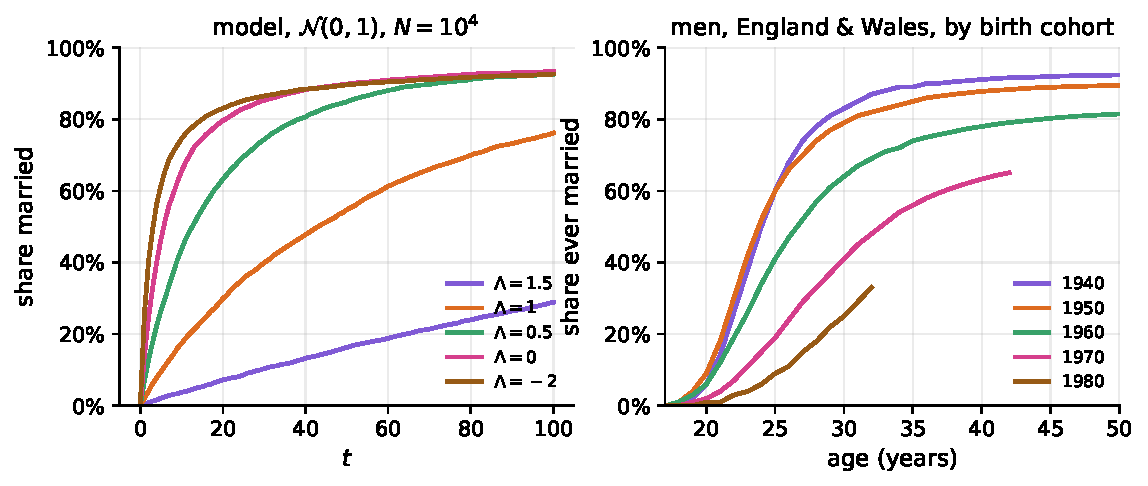
\includegraphics[width=\linewidth]{fig08_married_share}
  \caption{Left: share of married agents in the Gaussian model with
  $N = 10{,}000$ at each step, for $\Lambda = 1.5, 1, 0.5, 0, -2$ from the
  bottom line upwards. Right: share of men in England and Wales ever married by
  a given age, for the birth cohorts $1980, 1970, 1960, 1950, 1940$ from the
  bottom line upwards~\cite{owidmarriagesanddivorces}.}
  \label{fig:mc}
  \Description{Two panels of rising, saturating curves with similar shape; the
  model curves on the left and cohort data on the right.}
\end{figure}

The agreement is arguably good, given how much the model deliberately ignores---
divorce, most obviously. We note that divorce could be introduced by making
affinities time-dependent, as discussed below. We also stress that the
resemblance was not built into the matching process in any way: it is a purely
dynamical consequence.

Read through the model, the declining share of married men across cohorts
corresponds to a society-wide shift to higher $\Lambda$. This agrees with rough
expectations. In the past marriage was enforced by tradition and many couples
married without high affinity; progressive movements weakened those forces and
people became more demanding. If one goes further and associates each cohort
with the value of $\Lambda$ drawn in the same colour, then Figure~\ref{fig:lcomp}
implies that average utility with respect to relationships rose from 1940 to
1970 and perhaps began to fall from 1970 to 1980. If approximately correct, this
would suggest that progressive movements improved the matching market of
traditional societies by raising $\Lambda$---but that $\Lambda$ may since have
gone too high and need rebalancing, in the direction the advice of
Section~\ref{sec:results} points.

Two caveats. First, steps are not years. The model's curve is concave from
$t = 0$, whereas the data is S-shaped, because nobody marries before their late
teens; if the initial steps are compressed, as is reasonable, the convexity of
the early data is recovered. Any quantitative cohort-to-$\Lambda$ mapping needs
an explicit step-to-age map, which we do not have. Second, the association of
cohorts with particular $\Lambda$ values in Figure~\ref{fig:mc} is a visual one,
not a fit. Making it quantitative is the most promising route to the model's
main empirical payoff: a way to access an unobservable property of a society,
average utility with respect to relationships, through an observable one.

\subsection{An Operational Rule for an Agent}

To close, an operational answer to the question that opened the paper. The
affinity matrix contains information that is not accessible to the agents: they
discover an affinity only when they meet. An agent therefore does not know
$\sigma$ in advance. But it can use the utilities attained in previous matches to
estimate a mean and a spread, and use those estimates to decide. Given utilities
$\{u_t : 0 \leq t \leq T\}$, an agent should propose marriage at step $T+1$ if
%
\begin{align}
  u_{T+1} > \frac{1}{T}\sum_{t=0}^T u_t
  + \sqrt{\frac{1}{T}\sum_{t=0}^T u_t^2
    - \Big(\frac{1}{T}\sum_{t=0}^T u_t\Big)^2} .
  \label{eq:rule}
\end{align}
%
It is left to the agent to estimate correctly its affinity with the agents it has
already met. This is by no means a simple task, as we so commonly fool ourselves
in matters of love; perhaps it is not even a well-defined quantity.

%%%%%%%%%%%%%%%%%%%%%%%%%%%%%%%%%%%%%%%%%%%%%%%%%%%%%%%%%%%%%%%%%%%%%%%%

\section{Discussion and Limitations}
\label{sec:limitations}

It is important to emphasise that the benefits of marriage disclosed by this
model may be irrelevant once other aspects of marriage are considered. There are
many layers of our preferences concerning relationships that the model does not
represent, and Section~\ref{sec:who} shows that even within the model the
benefit is not uniform across agents.

A salient simplification is that affinities are time-independent. Making them
time-dependent would bring divorce into the model for free: given a married
couple, their affinity may fall below $\Lambda$, at which point they unmarry and
may break apart if one of them finds another mate. Time-dependent affinities
would also account for the spontaneous break-up of couples, which requires only
that the affinity fall below one partner's utility of being single. Understanding
the average dynamical behaviour of affinity between agents is beyond the scope of
this paper, but it is the single extension most likely to connect the model to
further data, such as divorce rates.

\balance

Three further limitations are worth naming. The matching process is uniform over
the whole society, whereas real meeting is strongly assortative by geography,
education and social network. The threshold $\Lambda$ is exogenous and uniform,
whereas Section~\ref{sec:who} suggests agents have heterogeneous incentives to
choose it. And the mean-field theory of Section~\ref{sec:largeN}, as currently
formulated, is exact only for the first step.

%%%%%%%%%%%%%%%%%%%%%%%%%%%%%%%%%%%%%%%%%%%%%%%%%%%%%%%%%%%%%%%%%%%%%%%%

\section{Conclusions}

We proposed and studied an agent-based model of mate searching and marriage in
large societies, built on a stochastic matching process and simple behavioural
rules. Investigating it discloses some benefits of marriage as a search
strategy. Most significantly, the average utility of a society with marriage can
be higher than that of a society without it, with an optimum near
$\Lambda \approx \sigma$; and marriage simultaneously compresses the
distribution of outcomes. We summarised these results as what sounds like good
advice: do not marry the first person you like and do not search for the love of
your life, but get married if you like your partner more than a sigma above
average.

We also showed that this benefit is not uniform. Once agents differ in
desirability by more than sampling noise, the gain accrues to the less
desirable, and beyond a moderate spread the most desirable agents are made
strictly worse off. Marriage in this model is insurance against being left, and
those never at risk of being left pay for it without needing it.

The average utility attained by the dynamics is well below that of a stable
matching computed by Gale--Shapley, which can be taken as a simulation-based
argument for a central mechanism---perhaps an application---with the information
to coordinate the marriage market. To test the adequacy of the model for real
societies we compared the evolution of the fraction of married agents with
cohort data and obtained good agreement. Finally, we formulated the model in the
limit of an infinite number of agents, derived the stationary distribution of
married couples in closed form for arbitrary affinity distributions, and
determined where the mean-field evolution equations are and are not valid.

This work leaves many directions open. For those with a mathematical bent, it
would be valuable to derive the corrected large-$N$ evolution equations by
tracking the joint density of a couple, and to prove that they are the true
limit. For those interested in the adequacy of the model, a more systematic
comparison between the fraction of couples in the model and in real societies is
needed, together with a mapping between steps and chronological time; with such
a mapping one could infer $\Lambda$ for a given society and, combined with
Figure~\ref{fig:lcomp}, advise it to be more or less selective. For those
interested in the mechanism design question, Section~\ref{sec:who} raises the
issue of whether a society-level $\Lambda$ is self-enforcing when agents differ
in desirability. And for those interested in perfecting the model, the
time-dependent affinity of Section~\ref{sec:limitations} is the natural next
step.

%%%%%%%%%%%%%%%%%%%%%%%%%%%%%%%%%%%%%%%%%%%%%%%%%%%%%%%%%%%%%%%%%%%%%%%%

\begin{acks}
This work was motivated by personal experiences with my girlfriend Lis, whom I
thank for her love and companionship. As I am sure that our affinities are more
than one sigma above the average, I hope the results presented here will convince
her that we should get married, as they have convinced me.
\end{acks}

%%%%%%%%%%%%%%%%%%%%%%%%%%%%%%%%%%%%%%%%%%%%%%%%%%%%%%%%%%%%%%%%%%%%%%%%

\bibliographystyle{ACM-Reference-Format}
\bibliography{bib}

\end{document}
